\chapter{Alkalmazások és kalibráció}
\section{Voltmérő}
Működés közben megjeleníti az akkumulátor feszültségét. Az evo\_v\_l számszerű értéket és akkumulátorjelet mutat; az iv\_evo\_v\_t az IV-Nano műszerhez hasonló szegmenses megjelenítést használ.

\begin{figure}[H]
\centering
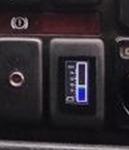
\includegraphics[width=.85\textwidth,height=.60\textheight,keepaspectratio]{figures/ivevo/image16.png}
\caption{Voltmérő}
\end{figure}

\begin{figure}[H]
\centering
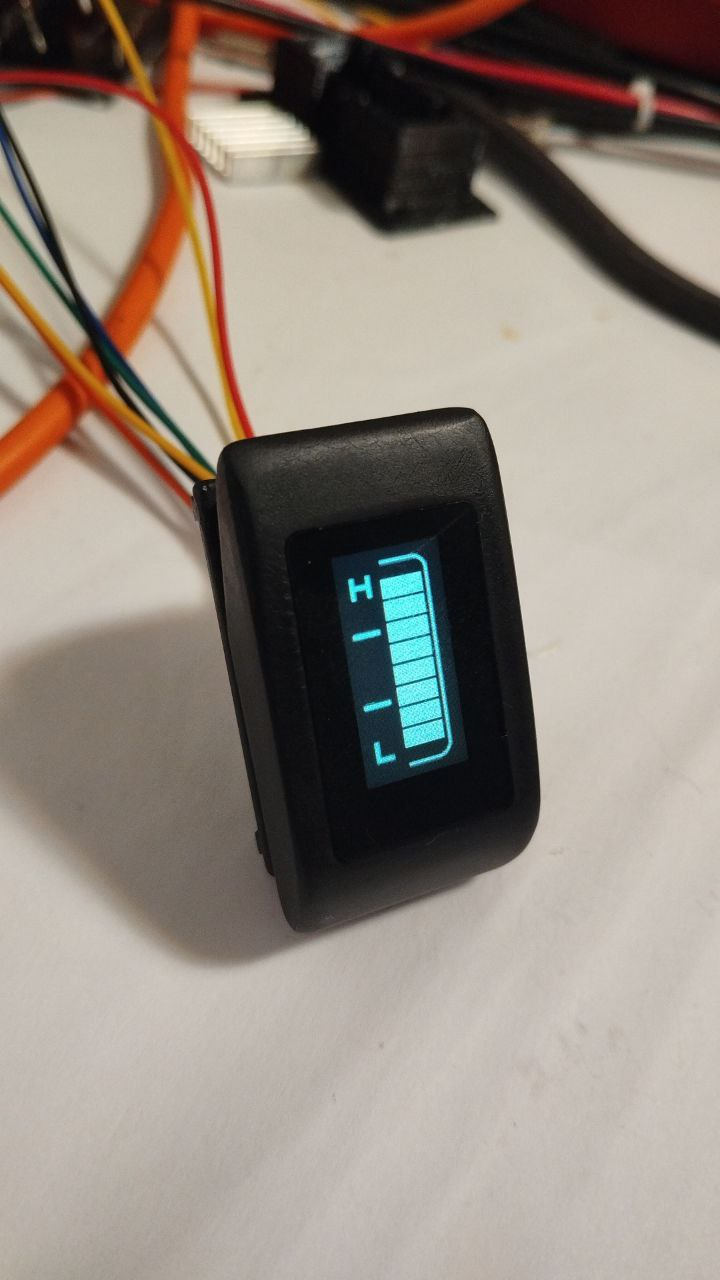
\includegraphics[width=.85\textwidth,height=.60\textheight,keepaspectratio]{figures/ivevo/image15.png}
\caption{Voltmérő}
\end{figure}

\begin{figure}[H]
\centering
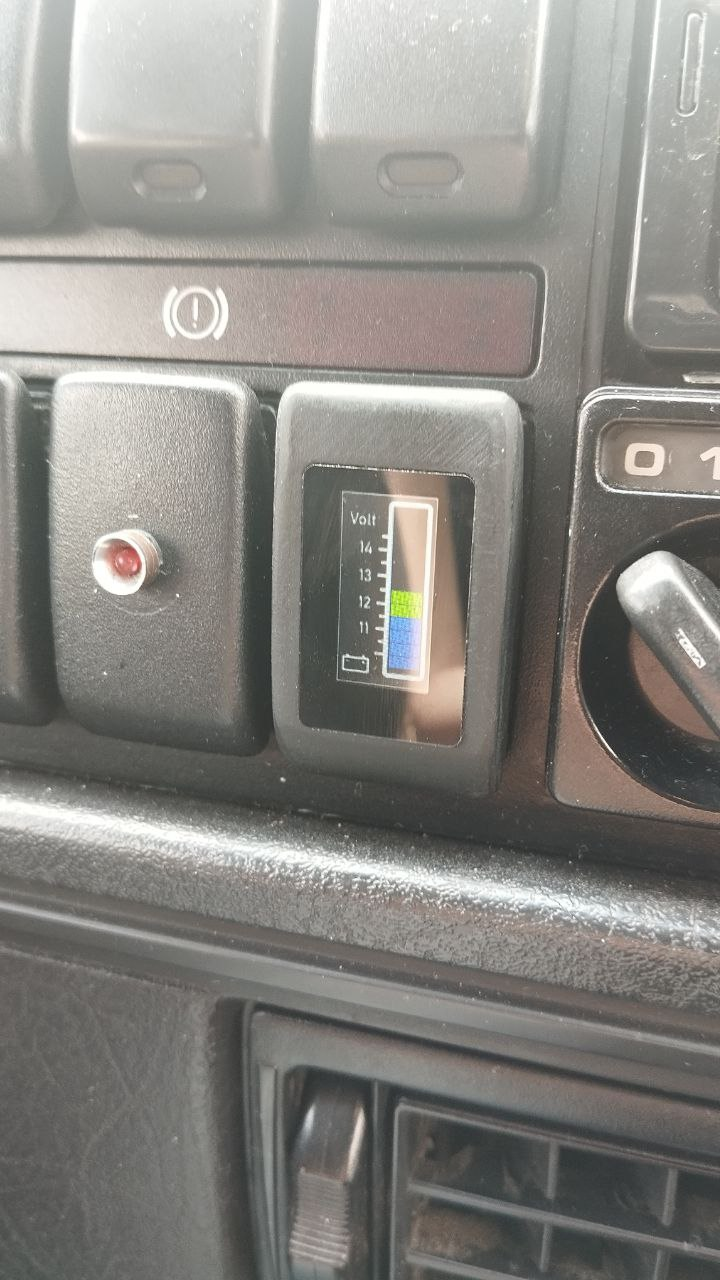
\includegraphics[width=.85\textwidth,height=.60\textheight,keepaspectratio]{figures/ivevo/image2.png}
\caption{Voltmérő}
\end{figure}
\section{Olajnyomás (Barometer)}
Érzékelő szükséges; az ajánlott típus VAG 03C906051A. Bár az IV-Evo rendelkezik belső +5 V-os kimenettel, a forrás külső DC/DC átalakítót ajánl az érzékelő táplálására. Kövesse az olajnyomás bekötési rajzát, és használjon az érzékelőhöz illő kalibrációt.

\begin{figure}[H]
\centering
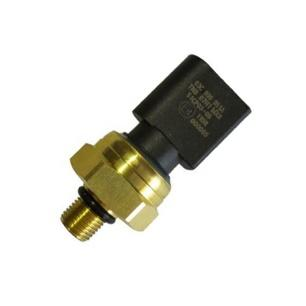
\includegraphics[width=.85\textwidth,height=.60\textheight,keepaspectratio]{figures/ivevo/image21.jpg}
\caption{Olajnyomás (Barometer)}
\end{figure}
\section{Hőmérséklet (Thermo)}
Válasszon NTC vagy digitális DS18B20 érzékelőt és a hozzá tartozó szkriptet. A kábeles DS18B20 szondák támogatottak. NTC-ként Ossca 01176 vagy kompatibilis Golf 2 érzékelő ajánlott. Az Ossca érzékelő 1-es és 2-es érintkezőjét össze kell kötni; az NTC ellenállás a 3-as érzékelőérintkezőre csatlakozik. Ezek az érzékelő számai, nem a kijelző tápérintkezői.

\begin{figure}[H]
\centering
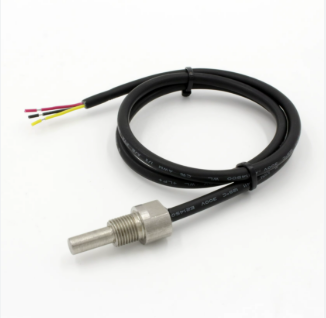
\includegraphics[width=.85\textwidth,height=.60\textheight,keepaspectratio]{figures/ivevo/image14.png}
\caption{Hőmérséklet (Thermo)}
\end{figure}

\begin{figure}[H]
\centering
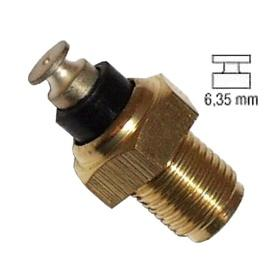
\includegraphics[width=.85\textwidth,height=.60\textheight,keepaspectratio]{figures/ivevo/image19.jpg}
\caption{Hőmérséklet (Thermo)}
\end{figure}
\section{Fokozatkijelző}
Az R és az 1–5 fokozat megjelenítésére alkalmas. A fokozatot a Digifiz Next által Bluetooth LE kapcsolaton küldött sebességből és fordulatszámból számolja. A hátramenetet a rajz szerinti bemenetre adott pozitív jel aktiválja. Digifiz Next 1.0.14 vagy újabb firmware szükséges.

Ennél az alkalmazásnál az 1-es érintkezőt (K30/KL30) a +12 V KL15 gyújtáskapcsolt tápra, a 7-est a jármű testpontjára csatlakoztassa. Induláskor a kötőjel azt jelzi, hogy nincs kiválasztott fokozat; a készülék keresi a Digifiz Next műszert. QR-kódos módban válassza az iv\_gear alkalmazást és a volts1 érzékelőt, mentse a beállítást, majd indítsa újra gyújtással.

A Digifiz Next webes felületén a sebességet GPS alapján, a fordulatszámot és a fokozattáblázatot pedig a járműhöz igazítva kalibrálja. A forrás 80–100 km/h sebességet javasol viszonyításra; ezt csak szabályos és biztonságos körülmények között végezze, az értékeket utas rögzítse. Az 1500, 3000 és 400 fordulatszám-kalibrációs értékek mértékegysége és motortípushoz rendelése nem egyértelmű. Ne találgasson: kövesse az adott motorra vonatkozó műszeregység-útmutatót.

\begin{figure}[H]
\centering
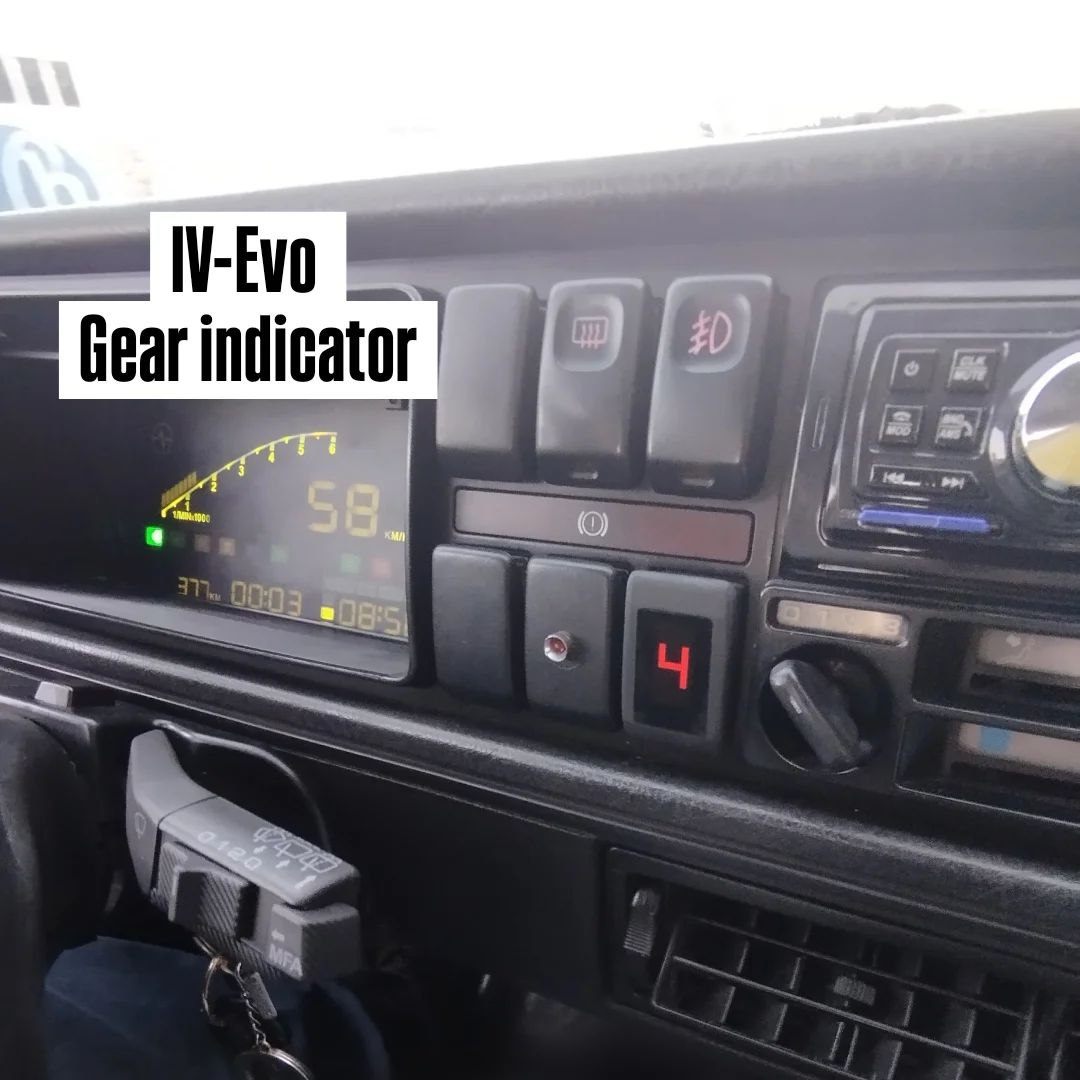
\includegraphics[width=.85\textwidth,height=.60\textheight,keepaspectratio]{figures/ivevo/image18.png}
\caption{Fokozatkijelző}
\end{figure}

\begin{figure}[H]
\centering
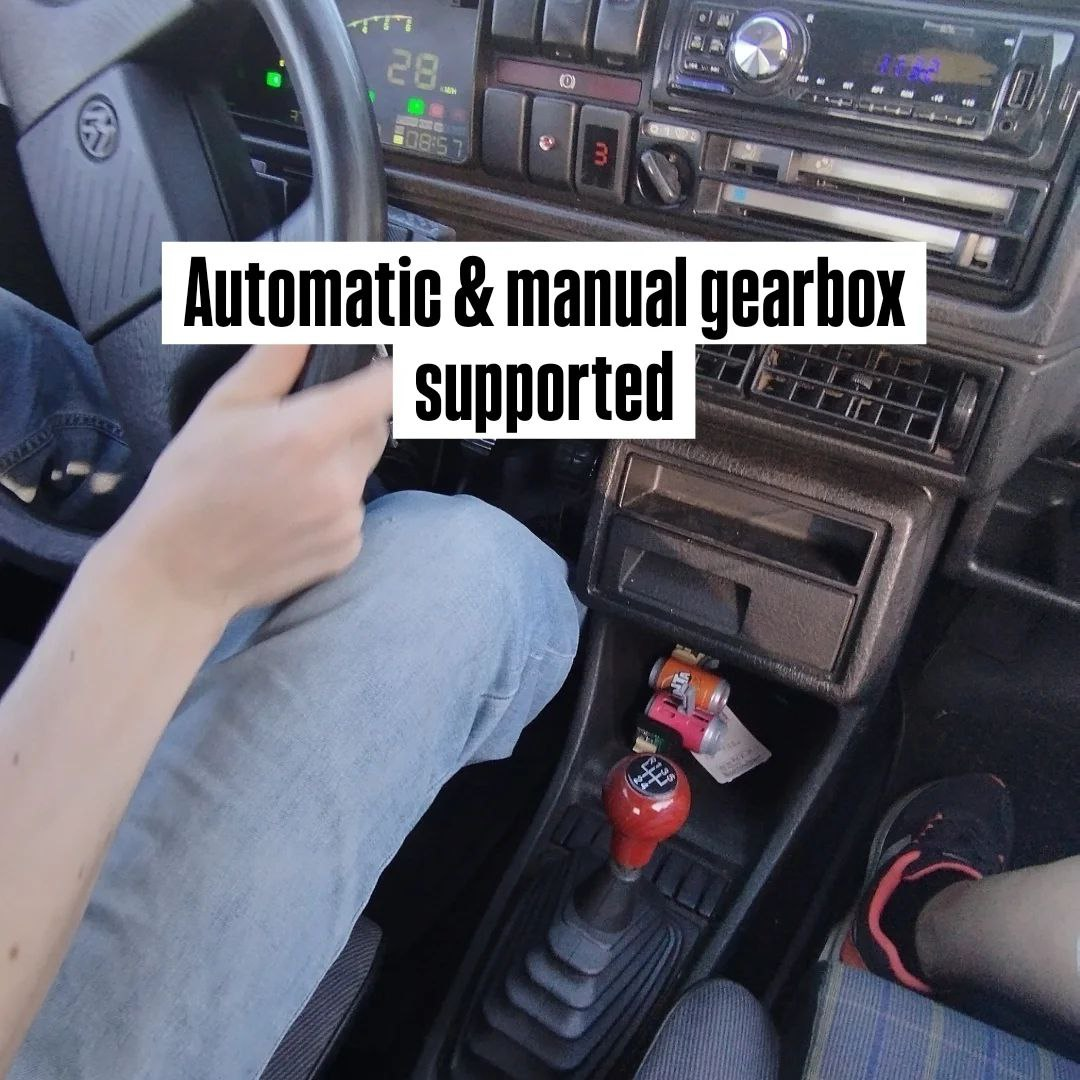
\includegraphics[width=.85\textwidth,height=.60\textheight,keepaspectratio]{figures/ivevo/image10.png}
\caption{Fokozatkijelző}
\end{figure}
\section{Lambda}
Ne csatlakoztassa a műszert a Golf 2 gyári lambdaszondájához. A forrás külön mérőszondát ír elő; a gyári szonda megtartása esetén két szonda lesz a járműben. A keskenysávú szonda körülbelül 0,1 V-ot ad szegény és 0,9 V-ot dús keveréknél, de nem mér pontos levegő–üzemanyag arányt. Közvetlen csatlakoztatása kalibrációt igényel.

A szélessávú szondának saját vezérlő kell; az IV-Evo nem képes közvetlenül vezérelni. Bosch LSU 4.9 ajánlott kompatibilis vezérlővel, például SLC Free, DIY-EFI TinyWB, Sigma Lambda Controller Free 2 vagy rusEFI wideband. A szondát a vezérlő útmutatója szerint kösse be, majd annak analóg kimenetét használja. Ez lehet 0–5 V, 0,5–4,5 V vagy 0–1 V; a bemeneti átszámításnak és a kalibrációs görbének ehhez kell illeszkednie.

\begin{figure}[H]
\centering
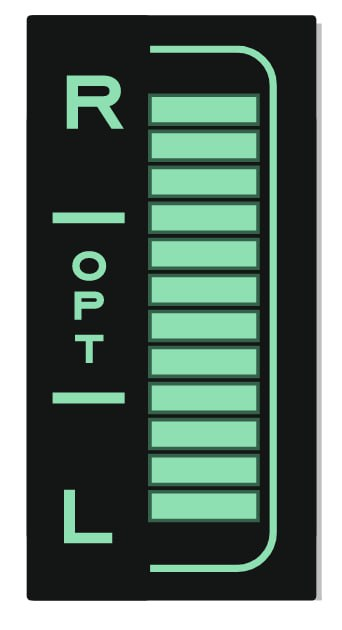
\includegraphics[width=.85\textwidth,height=.60\textheight,keepaspectratio]{figures/ivevo/image7.png}
\caption{Lambda}
\end{figure}
\section{Check Engine}
A 2-es érintkezőn (V2) 12 V esetén „Check Engine” felirat jelenik meg, 0 V-nál üres a kijelző. Ez jelzésmegjelenítő, a forrás nem ír le hibakódolvasást vagy OBD-felületet.

\begin{figure}[H]
\centering
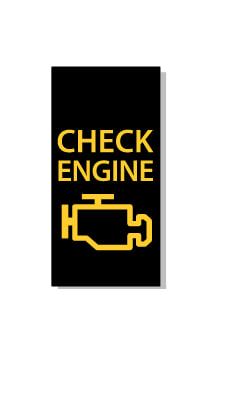
\includegraphics[width=.85\textwidth,height=.60\textheight,keepaspectratio]{figures/ivevo/image4.png}
\caption{Check Engine}
\end{figure}
\section{Töltőnyomás (Boost)}
A leírt érzékelő hárompólusú, +5 V tápfeszültségű, egy rögzítőfurattal rendelkezik, mérési tartománya 20–250 kPa. Névleges kimenete +1,8 V. Az ehhez tartozó nyomás és a teljes átviteli függvény nincs megadva. Kalibrálás előtt azonosítsa a pontos érzékelőt és annak jelleggörbéjét; egyetlen értékből ne következtessen a meredekségre.

\begin{figure}[H]
\centering
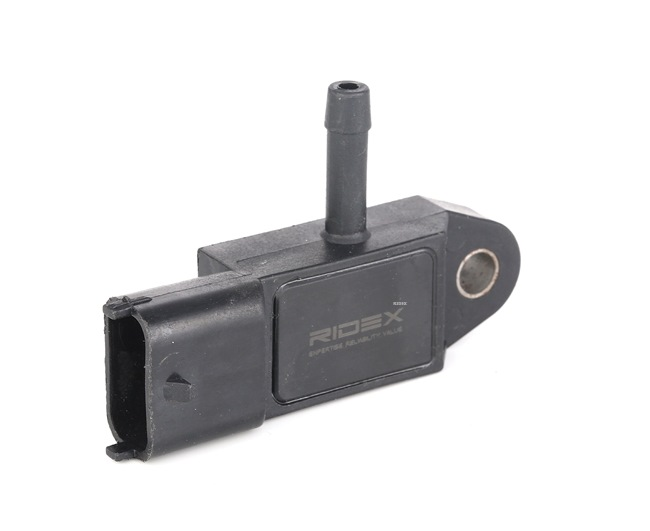
\includegraphics[width=.85\textwidth,height=.60\textheight,keepaspectratio]{figures/ivevo/image9.png}
\caption{Töltőnyomás (Boost)}
\end{figure}
\section{Óra}
A példaalkalmazás a rendszerórát használja. Az idő újraindításkor nem marad meg, ezért újbóli beállítás nélkül menetidő-kijelzőként működik.

\begin{figure}[H]
\centering
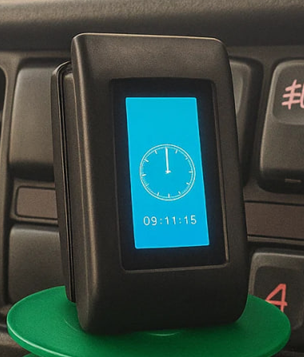
\includegraphics[width=.85\textwidth,height=.60\textheight,keepaspectratio]{figures/ivevo/image12.png}
\caption{Óra}
\end{figure}
\section{A dokumentáció korlátai}
Nincs megadva általános tápfeszültség-tűrés, üzemi hőmérséklet-tartomány vagy a ház védettsége. Ne alkalmazza a Nano adatait az IV-Evo készülékre.
